\begin{tikzpicture}
\draw[-latex] (0,0) -- (15,0);
\draw[-latex] (0,0) -- (0,15);
\foreach \x in {1,2,...,14} {
  \draw (\x,0.1) -- (\x,-0.1);
  \draw (-0.1,\x) -- (0.1,\x);
}
%\draw (2,3) -- (10,6) -- (11,11) -- (3,10) -- (2,3);
\node at (12,3) {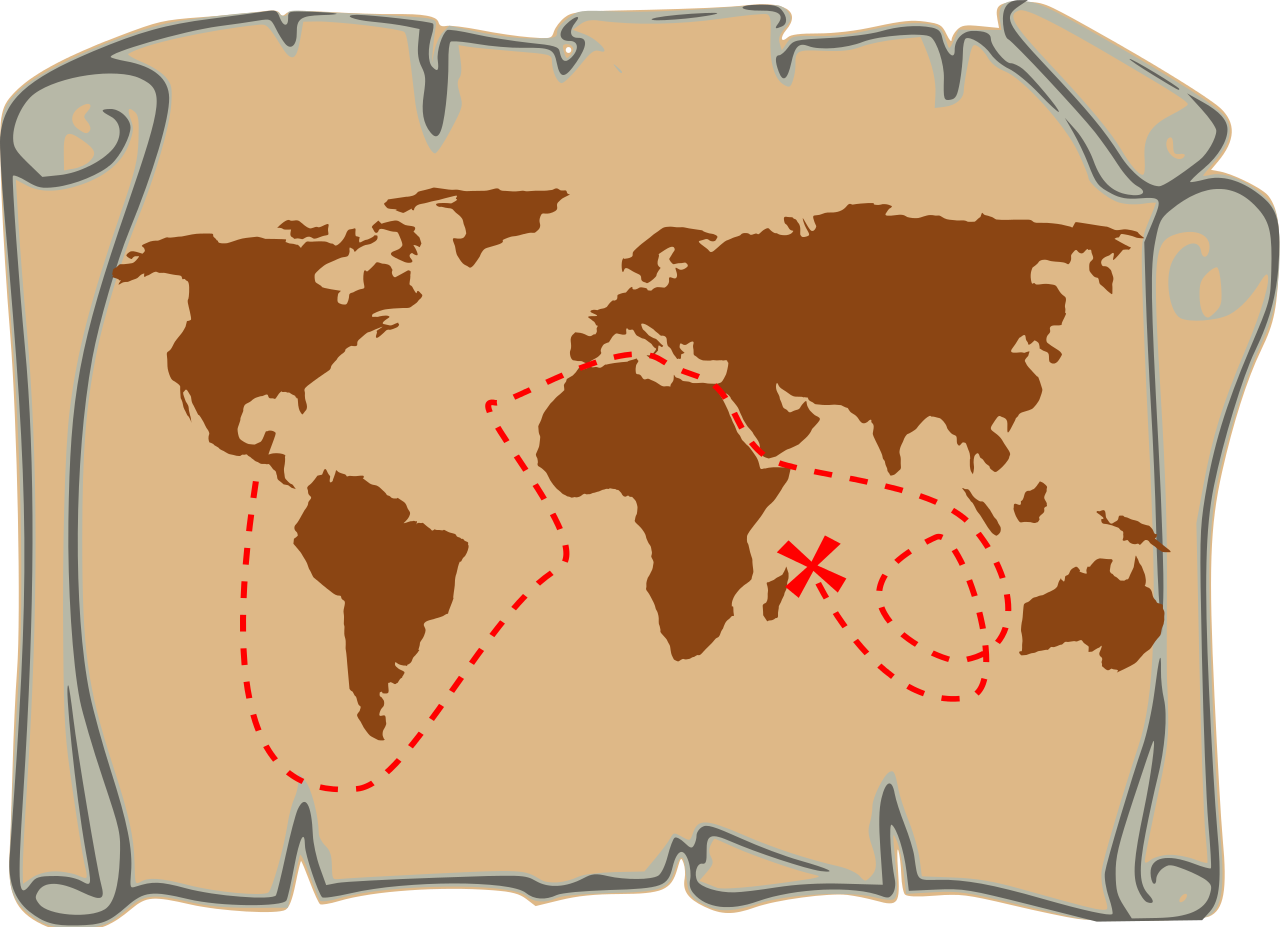
\includegraphics[width=1in]{assets/clipart/map.png}};
\node at (4,6) {
\includegraphics[width=1in]{assets/clipart/hat.png}};
\node at (8,8) {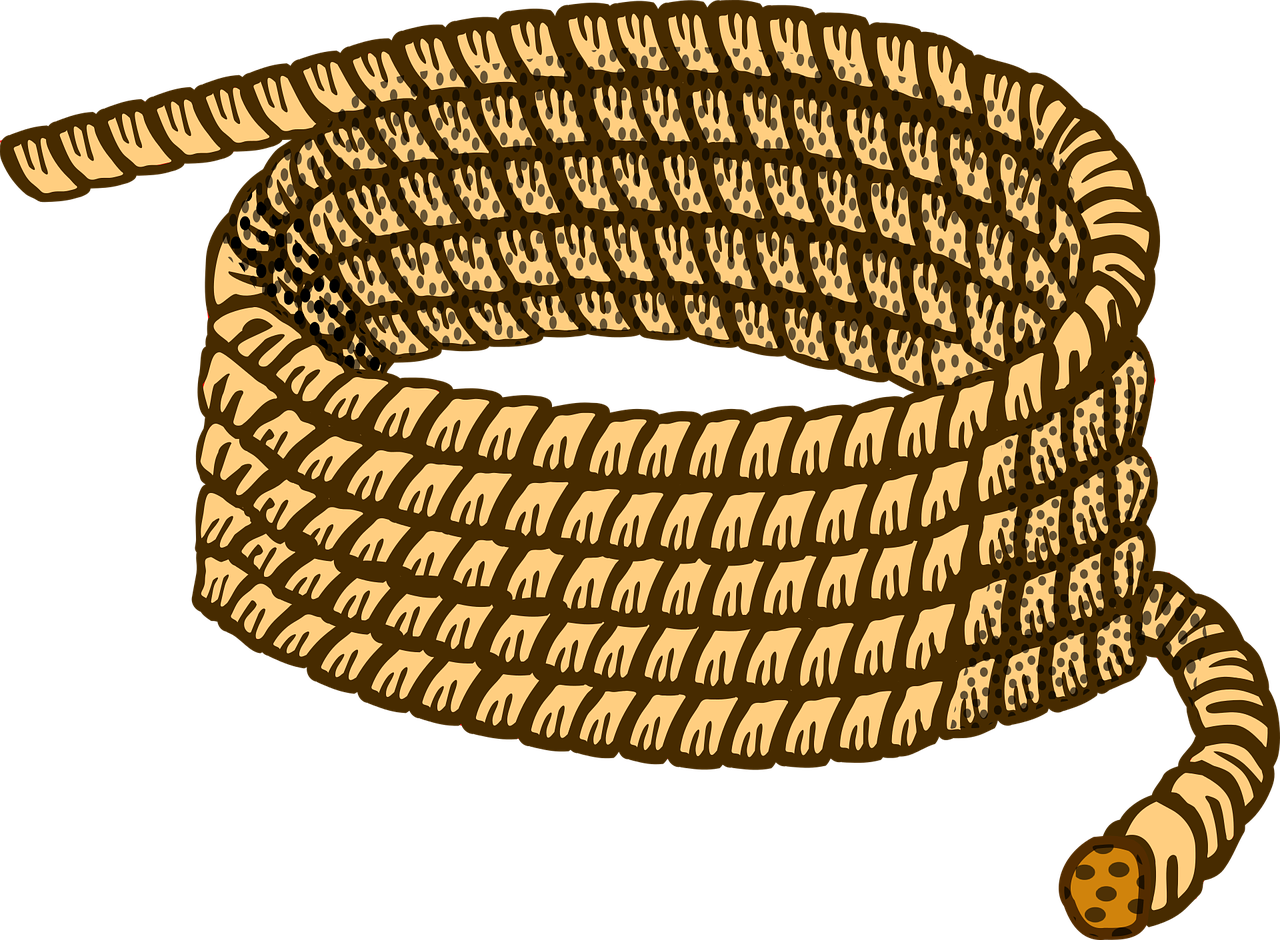
\includegraphics[width=1in]{assets/clipart/rope.png}};
\node at (3,12) {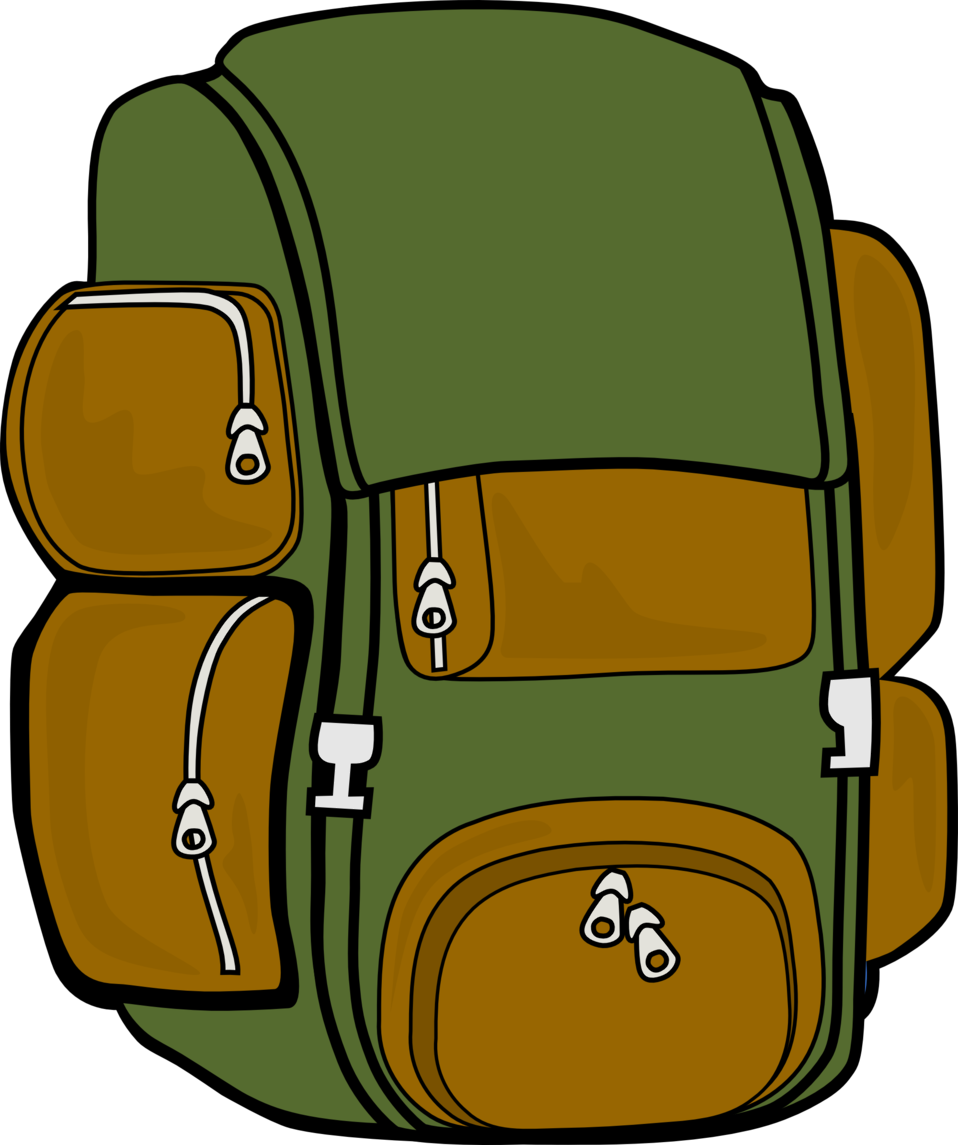
\includegraphics[width=1in]{assets/clipart/backpack.png}};
\node at (13,7) {
\includegraphics[width=1in]{assets/clipart/compass.png}};
\node at (7,2) {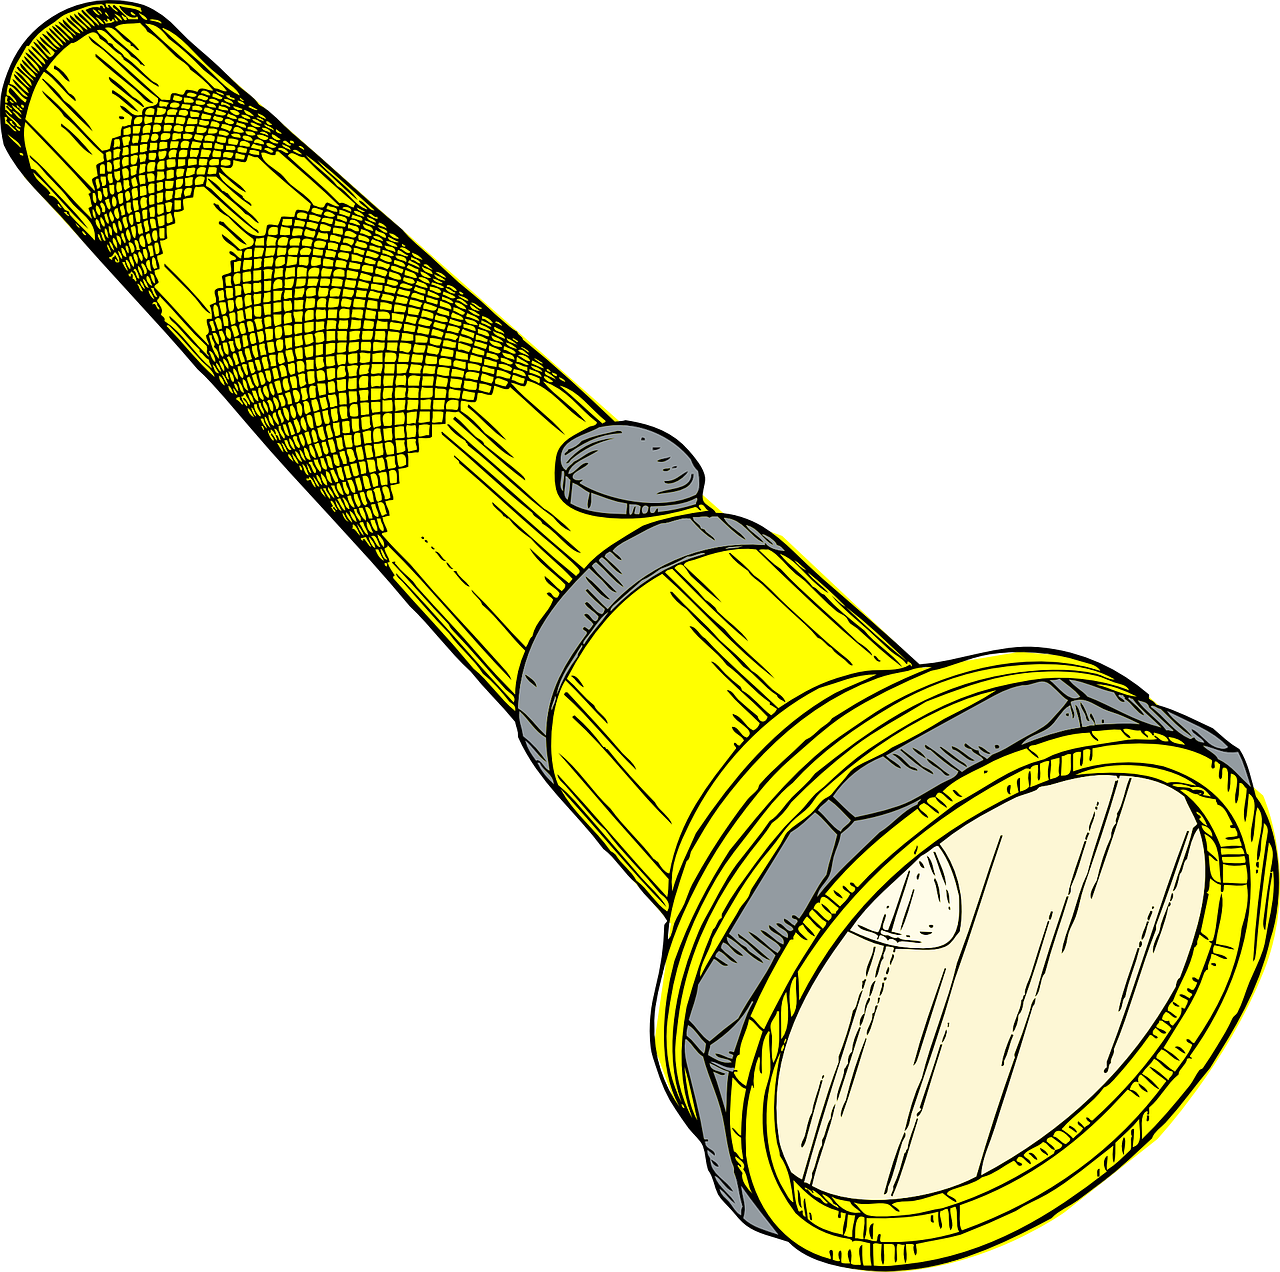
\includegraphics[width=1in]{assets/clipart/flashlight.png}};
\end{tikzpicture}

TODO: In cluekeeper players are told to connect the coordinates
given by the previous puzzle to encircle two of the objects in
the figure. (for now, these are (2,3) (10,6) (11,11) (3,10)).
They are also told that the correct password is the combination
of two of the following words: 
BACKPACK, COMPASS, FLASHLIGHT, HAT, MAP, ROPE.
